\chapter{Introduction} \label{chap:intro}

\section*{}

%O primeiro capítulo da dissertação deve servir para apresentar o enquadramento e a moti\-va\-ção do trabalho e para identificar e definir os problemas que a dissertação aborda. Deve resumir as metodologias utilizadas no trabalho e termina apresentando um breve resumo de cada um dos capítulos posteriores.

%Like the Abstract, the Introduction should be written to engage the interest of the reader. It should also give the reader an idea of  how the dissertation is structured, and in doing so, define the thread of the contents.

Once more, a technological revolution sparked in a not-yet-ready world. Just as the Internet invention brought us closer together and opened an unlimited virtual world of possibilities so does blockchain. The technology is still in it's early development days and many different proposals are being worked on as to improve it's performance and scalability. Akin to the dotcom boom, a plethora of blockchain projects live on more expectations than results but ultimately blockchain could resolve the Internet's failed promise. To understand what is blockchain and why it is necessary we need to comprehend the social background around the time of its release. The Internet promised of a peer-to-peer connected world, however, financial incentives and technological challenges led to a centralized and non-privacy advocated virtual world. The increasing general concern regarding privacy of personal information and the meddling of third parties in everyday online actions allied with the financial crash of 2008 lead to a new technological and social breakthrough.

Satoshi Nakamoto's introduced Bitcoin, in 2009~\cite{Nakamoto2009Bitcoin:System}, and revolutionized money and currency, setting the first example of a digital asset which has no backing or intrinsic value and more importantly no centralized issuer or controller. In order to require no third party to verify each transaction and prevent double-spending, he introduced a distributed ledger mechanism now known as Blockchain.

\section{Blockchain}

Blockchain is a tool for distributed consensus, in a byzantine fault-tolerant approach, without requiring to trust in centralized parties. In this ledger, transactions are recorded in an ongoing chain, creating an immutable public record that cannot be changed without redoing the proof-of-work. Anyone can become a node and leave and rejoin the network. Having incentives to work on the CPU intensive proof-of-work, extending the chain, and so, for as long as the majority of nodes are trustworthy, the longest and honest chain will thrive. The proof-of-work used on Bitcoin is HashCash, proposed in 1997 by Adam Back, is a cryptographic hash-based proof-of-work algorithm that requires a selectable amount of work to compute, but the proof can be verified efficiently. Nodes can easily verify that a block is valid and that some effort was put in its creation. The proof-of-work difficulty can increase and decrease depending on the network size and capability, creating on average a block every 10 minutes, like an heartbeat.

In simpler terms, transactions are grouped in blocks and for each block there is a mathematical challenge (proof-of-work) which requires time and computational resources to be solved, guaranteeing that some effort is put into solving the challenge and therefore making it extremely hard to quickly manufacture false blocks. Each block has an hash, a signature, of the previous block linking all blocks in a single chain. Nodes always work on the longest chain, so as long as the majority of the nodes are honest and work in building correct blocks, which means they don't have double entries and transactions are legitimate, the biggest chain will will grow and remain a trusted and distributed ledger.

Leveraging Blockchain, Bitcoin requires no personal information to exchange value, anyone can join the network and no central authority is needed. This opens an unlimited world of new scenarios for the use of blockchain.



\section{Smart Contracts}

In 2015, Ethereum was launched as an alternative protocol for building decentralized applications called smart contracts. Introduced as applications that run on the blockchain, smart contracts are self-verifying, self-executing and immutable contracts whose terms are directly written in lines of code which persist on the blockchain, promising to replace real world contracts. Contracts are the building blocks of our identity, economy and society. They enforce agreements between multiple parties and ensure trust in the compliance of the rules of the agreement but traditional contracts lack on automation and decentralization. Smart Contracts provide the ability to execute tamper-proof digital agreements, which are considered highly secure and highly reliable. 

Smart contracts have a wide range of use cases. For example, they can be used in Supply Chains and Logistics. Smart contracts allow tracking product movement from the factory to the store shelves. Each intermediary signs a step of the contract which then the final consumer can analyse and have the guarantee of the origin of the product.

\section{The smart contract connectivity problem}

\begin{figure*}[t]
  \begin{center}
    \leavevmode
    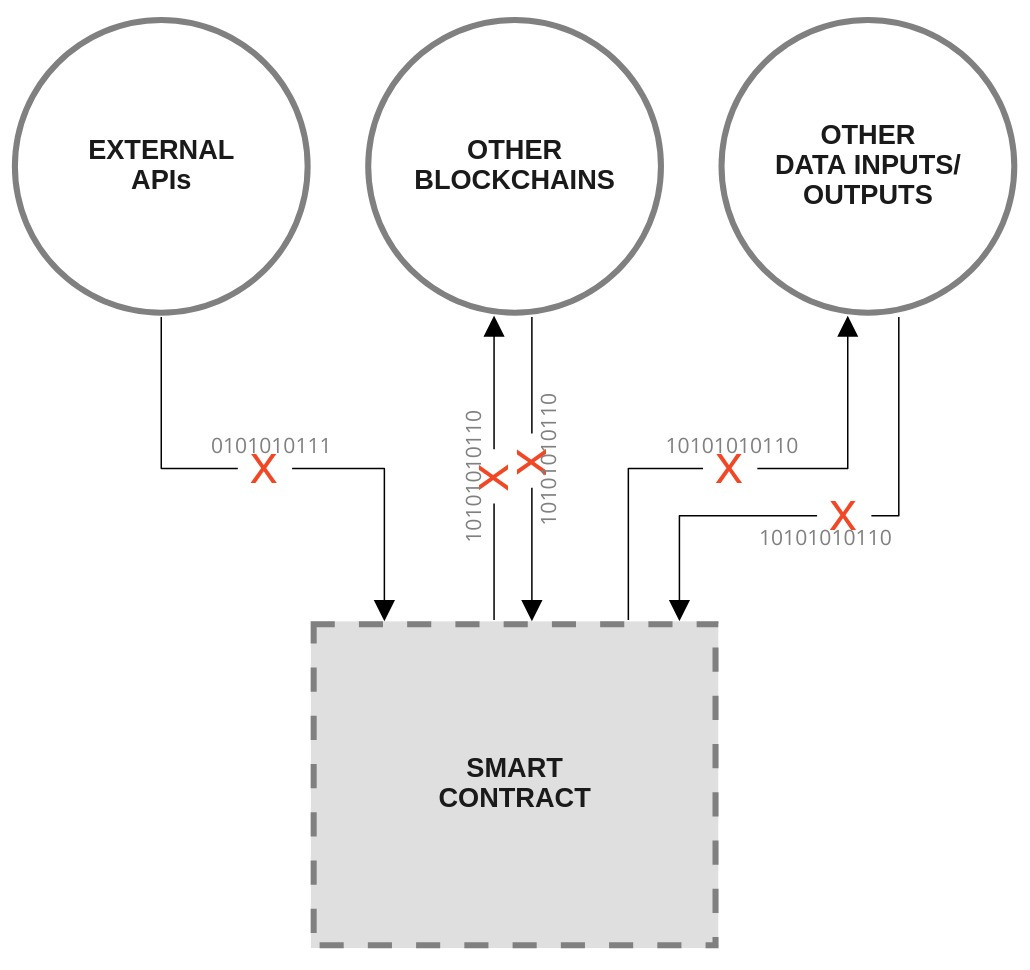
\includegraphics[width=0.7\textwidth]{figures/sc_connectivity.jpg}
    \caption{Smart contract connectivity problem.}
    \label{fig:/figures/sc_connectivity.jpg}
  \end{center}
\end{figure*}

The Ethereum blockchain is designed to be entirely deterministic~\cite{GavinWood2014Ethereum:Ledger}, meaning that if someone downloads the whole network history and replays it they should always end up with the same state. Bearing this in mind, smart contracts cannot directly query URLs for a certain information since everyone must be able to independently validate the outcome of running a given contract making it impossible to guarantee that everyone would retrieve the same information since the internet is non-deterministic and changes over time. Determinism is necessary so that nodes can come to a consensus. In order for smart contracts to gain traction they need access information of the real world, outside of the blockchain. For example, the current price of the US dollar. However smart contracts cannot directly query the internet for information due to the non-deterministic nature of the internet. Meaning that the information retrieved at some point in time cannot be entrusted to be available or equal in another point in the future, which may result in different states when validating smart contracts by querying the internet in different moments. Oracles solve the non-deterministic problem, of querying the internet, by inputting external information on the blockchain through a transaction making sure that the blockchain contains all the information required to verify itself. 



\section{Smart contracts space and computation limits}

Another problem for smart contracts is performing long and costly operations in terms of computation and space. Several platforms are implementing smart contracts, also called DAPPs, Distributed Applications, namely Ethereum and EOS, among others. 

On the Ethereum platform, smart contracts pay "Gas" to run. "Gas" is a unit that measures the amount of computation effort that certain operations require to execute. "Gas" is basically the fees paid to the network in order to execute an operation. Therefore, the longer the application runs the more "Gas" the smart contract as to pay.

EOS, on the opposite of Ethereum, works on an ownership model whereby users own and are entitled to use of resources in proportion to their stake. Basically, instead of paying transaction fees, the owner who holds N tokens is entitled to N*k transactions. While Ethereum rents out computational power on the network, EOS gives ownership of the resources in accordance to the amount of EOS held. The mentioned resources are RAM, corresponding to the used state on the network, CPU measuring the average consumption of computing resources and NET which measures used bandwidth. With increasing prices of EOS tokens, staking these resources becomes very costly.

All in all, either for users of smart contracts or the teams deploying them, keeping smart contracts efficient and performing non-costly operation is the key. Nonetheless, sometimes applications require costly operations and outsourcing them to an oracle outside of the blockchain is the answer.


\section{Oracles as a solution}
The solution to the smart contract connectivity problem and to outsourcing computation from the blokchain is the use of a secure blockchain middle-ware, mentioned before as, an oracle. Oracles can query data from APIs, datafeeds, other blockchains or perform their own calculations and input that data on the smart contract. This way the blockchain has all the necessary information to verify the result of running a smart contract, and will always produce the same result, independently of the point in time in which that verification is ran.


\begin{figure*}[t]
  \begin{center}
    \leavevmode
    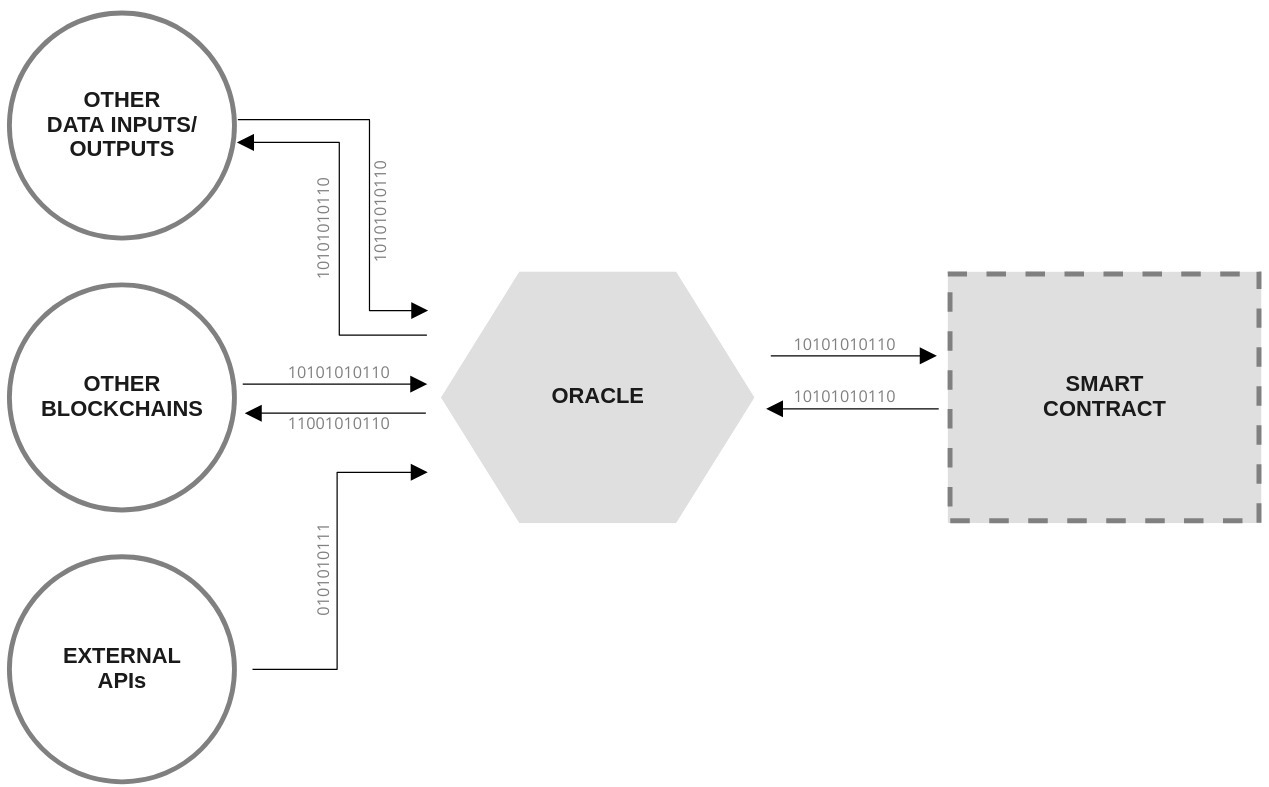
\includegraphics[width=\textwidth]{figures/oracle.jpg}
    \caption{Oracle integration.}
    \label{fig:/figures/oracle.jpg}
  \end{center}
\end{figure*}


\section{Oracles trust}
Trust in oracles comprises two main components, service availability, trusting that the service will always return a response to our query, and untampered relay of information, meaning the information the oracle computed or queried is original and not tampered with. If oracles are compromised we risk compromising the trust of the underlying blockchain by inputting falsified information in a system that is trusted to always have a valid state. Therefore it is imperative that oracles provide a proof for the information they provide, as well, as keep a decentralized approach by having a network of oracles always available to answer the queries.

\section{Motivation and Objectives} \label{sec:goals}
The research hereby exposed was proposed by Takai, a blockchain start-up born in Porto, Portugal with the purpose to be the first blockchain open innovation platform. Sponsored by Bright Pixel, an innovation hub and venture investment house, who supports promising startups in their early years. Taikai is building a platform that connects talent and entrepreneurs with the challenges of the corporate players, through the power of the sharing economy and blockchain trust. Taikai's project will serve as proof-of-concept for the implementation of trustable oracles.

The growing interest in blockchain technology and specially in the potential of Smart Contracts together with the lack of research on trustable oracles creates a gap on the general adoption of blockchain by business and governments. This gap and the opportunity bestowed with the Taikai project provides the perfect context for pursuing the construction of a bridge to overcome the oracle trust problem and further empower existing and future blockchain projects.

The proposed objectives for this work are as follows:
\begin{itemize}
\item Identifying the necessary components for end-to-end reliability between smart contracts and outside blokchain information;
\item Providing a general framework for guaranteeing oracle trust;
\item Implementing a proof-of-concept in the Taikai project on the EOS blockchain;
\end{itemize}

\section{Document Structure} \label{sec:struct}

%Para além da introdução, esta dissertação contém mais x capítulos.
%No capítulo~\ref{chap:sota}, é descrito o estado da arte e são
%apresentados trabalhos relacionados. 
%%\todoline{Complete the document structure.}
%No capítulo~\ref{chap:chap3}, ipsum dolor sit amet, consectetuer
%adipiscing elit.
%No capítulo~\ref{chap:chap4} praesent sit amet sem. 
%No capítulo~\ref{chap:concl}  posuere, ante non tristique
%consectetuer, dui elit scelerisque augue, eu vehicula nibh nisi ac
%est. 
